\documentclass[14pt]{beamer}
\usetheme{Montpellier}
\usepackage[utf8]{inputenc}
\usepackage[english]{babel}
\usepackage{amsmath}
\usepackage{amsfonts}
\usepackage{amssymb}
\usepackage{graphicx}
\usepackage{enumitem}
\usepackage{lmodern}

\author{Oumaima Al Qoh, Francisco Arrieta, Lucia Camenisch, Manuela Giansante, Emily Schmidt, Camille Beatrice Valera}
\title{Case Study B \\ Pain Relief Medication}
\date{April 28, 2023} 
%\subject{}
%\logo{}
%\institute{}

  
\setbeamertemplate{navigation symbols}{
\usebeamerfont{footline}
\insertframenumber/\inserttotalframenumber
}



\begin{document}


\begin{frame}
\titlepage
\end{frame}



\begin{frame}
\frametitle{Table of Contents}
\tableofcontents
\end{frame}


\section{Case Statement}
\begin{frame}
\frametitle{Case Statement}
\begin{itemize}[label={$\blacktriangleright$}]
\item 20 experiments on mice with combinations of marijuana and morphine, of which:
\begin{itemize}[label={$\blacktriangleright$}]
\item 1 control experiment;
\item 5 experiments with marijuana only;
\item 8 experiments with morphine only;
\item 6 experiments with both drugs.
\end{itemize}
\item 10 mice used per experiment;
\item Each mouse undergoes a tail flick test.
\end{itemize}
\end{frame}

\begin{frame}
The tail flick test assesses the effect of drugs on the mouse.

\bigskip

In each experiment, the proportion of mice not flicking their tail can be interpreted as a \textbf{measure of the effect of the drug} for the chosen experimental dosage.
\end{frame}

\section{Objectives}
\begin{frame}
\frametitle{First Objective}
\textit{Determine the minimum dosage amount of the drugs that achieves \textbf{efficacy}.}

\bigskip

The dosage of a drug is said to be \textbf{effective} if at least 50\% of the subjects are responding.
\end{frame}


\begin{frame}
\frametitle{Second Objective}
\textit{Detect whether a \textbf{synergy} exists between the two drugs.}

\bigskip

There is \textbf{synergy} between two drugs if for some dosages, the combined effect is greater that the effect both drugs would have if they were acting independently, without interaction.
\end{frame}


\section{Identifying Synergy with the Isobole Method}
\begin{frame}
\frametitle{Identifying Synergy with the Isobole Method}
The isobole method is a graphical representation which identifies synergy and helps to better understand the concept.

\bigskip

Before constructing the isobole, we must determine the dosage at which the efficacy is 50\% for both drugs used separately.
\end{frame}

\begin{frame}
\begin{center}
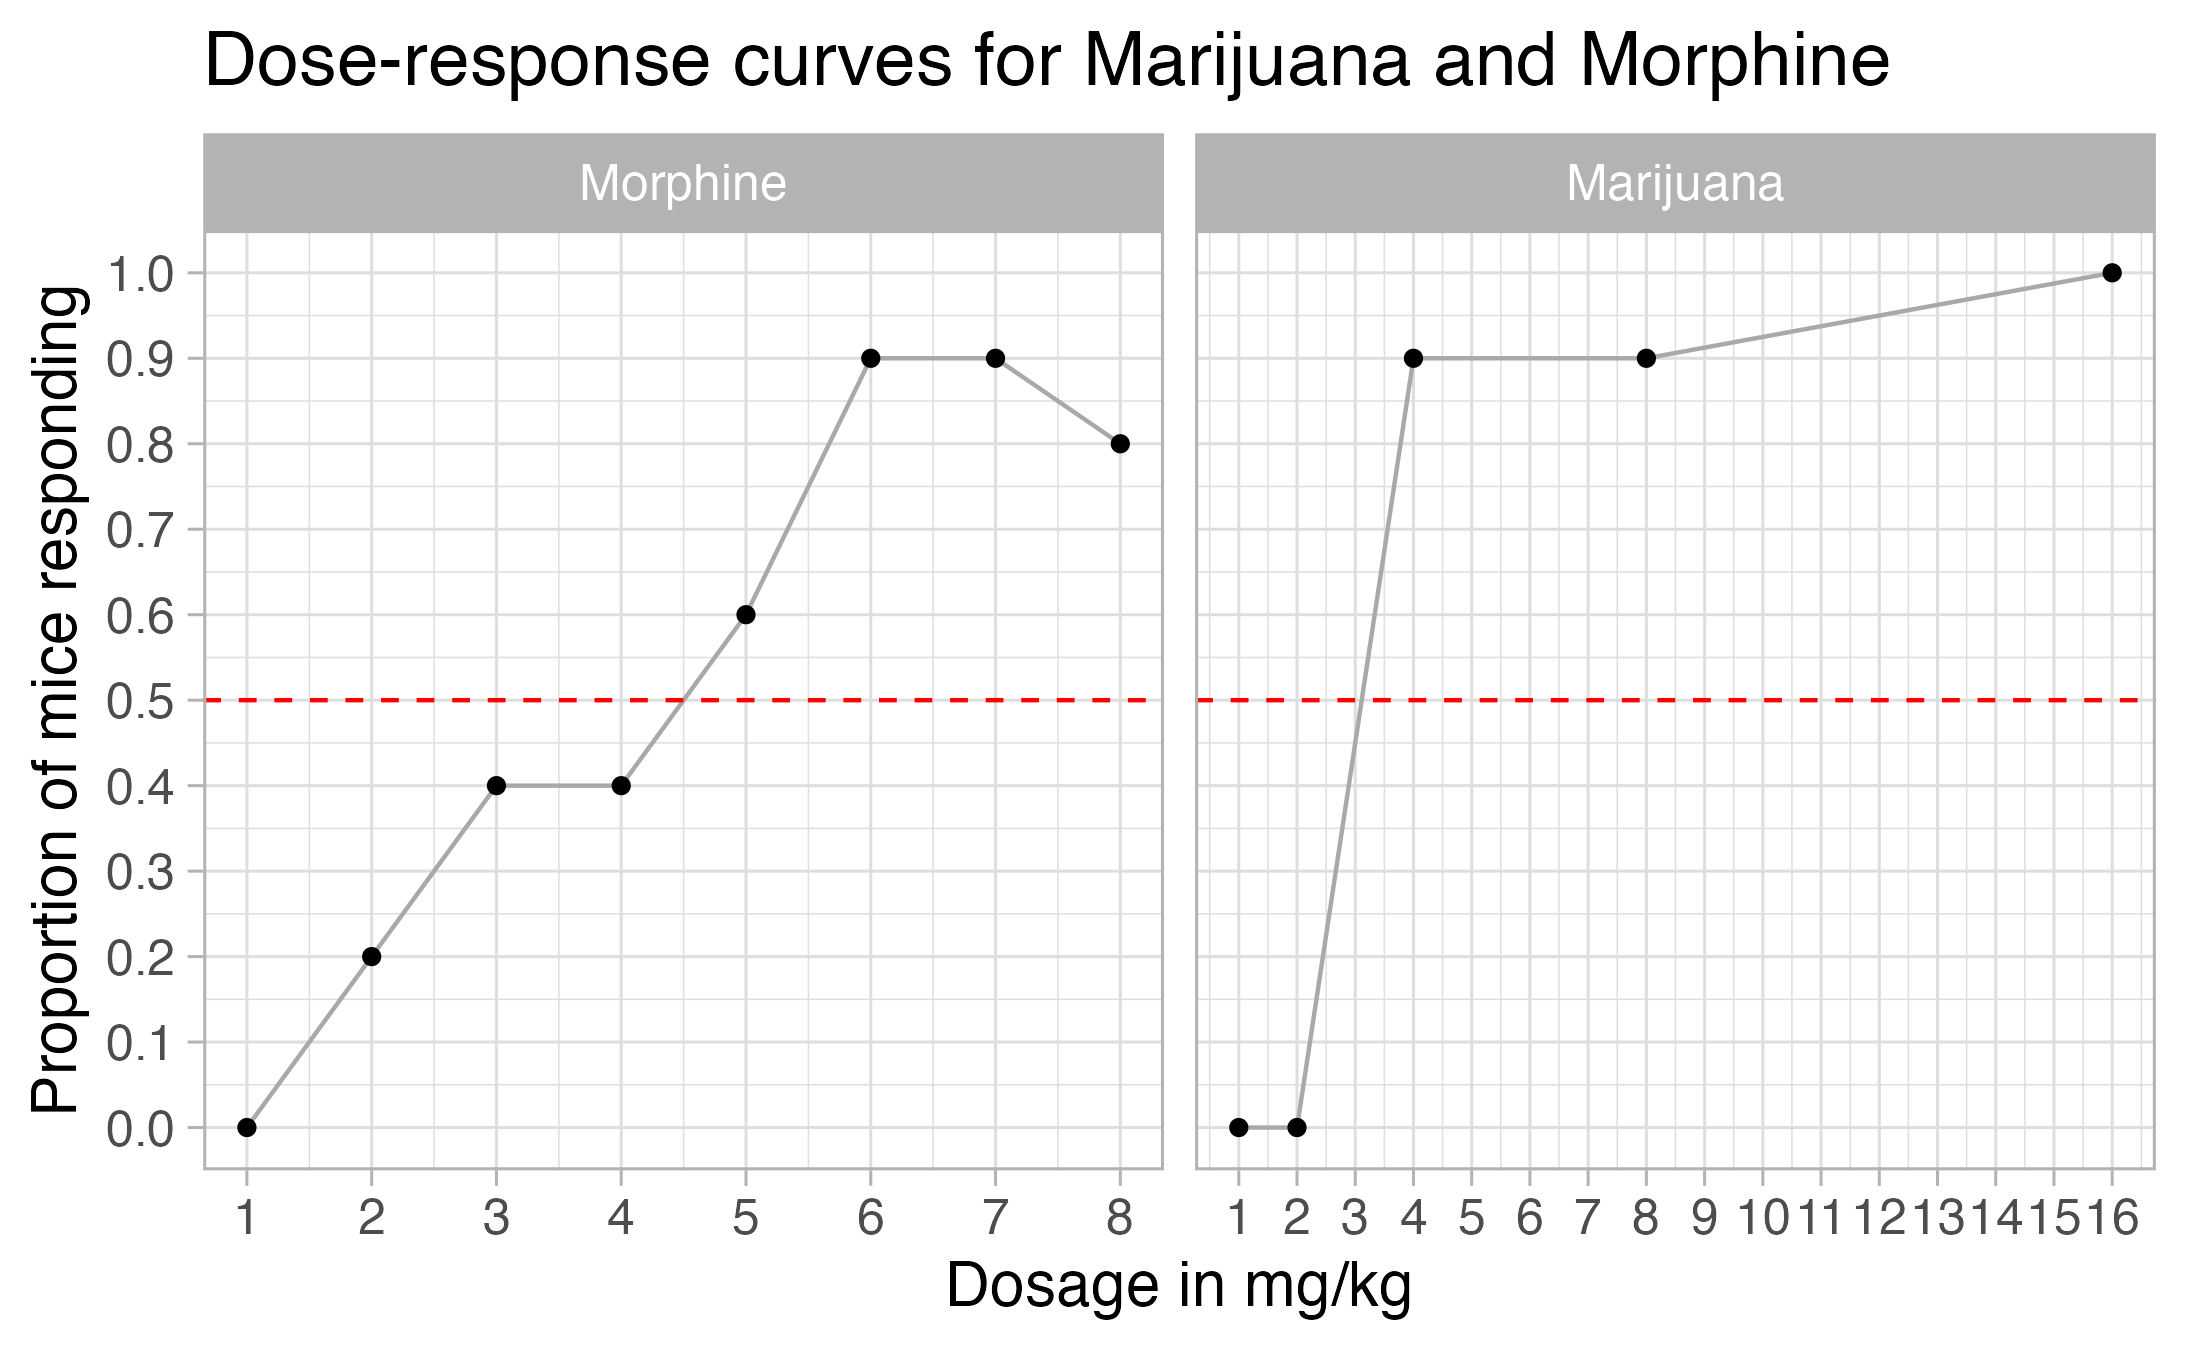
\includegraphics[scale=0.6]{dose-response.png}
\end{center}
\end{frame}

\begin{frame}
\textbf{Assumption:} The theoretical dosages which give a 50\% efficacy level are 
\begin{itemize}[label={$\blacktriangleright$}]
\item 3.0 mg/kg of marijuana;
\item 4.5 mg/kg of morphine.
\end{itemize}
\end{frame}

\begin{frame}
\begin{center}
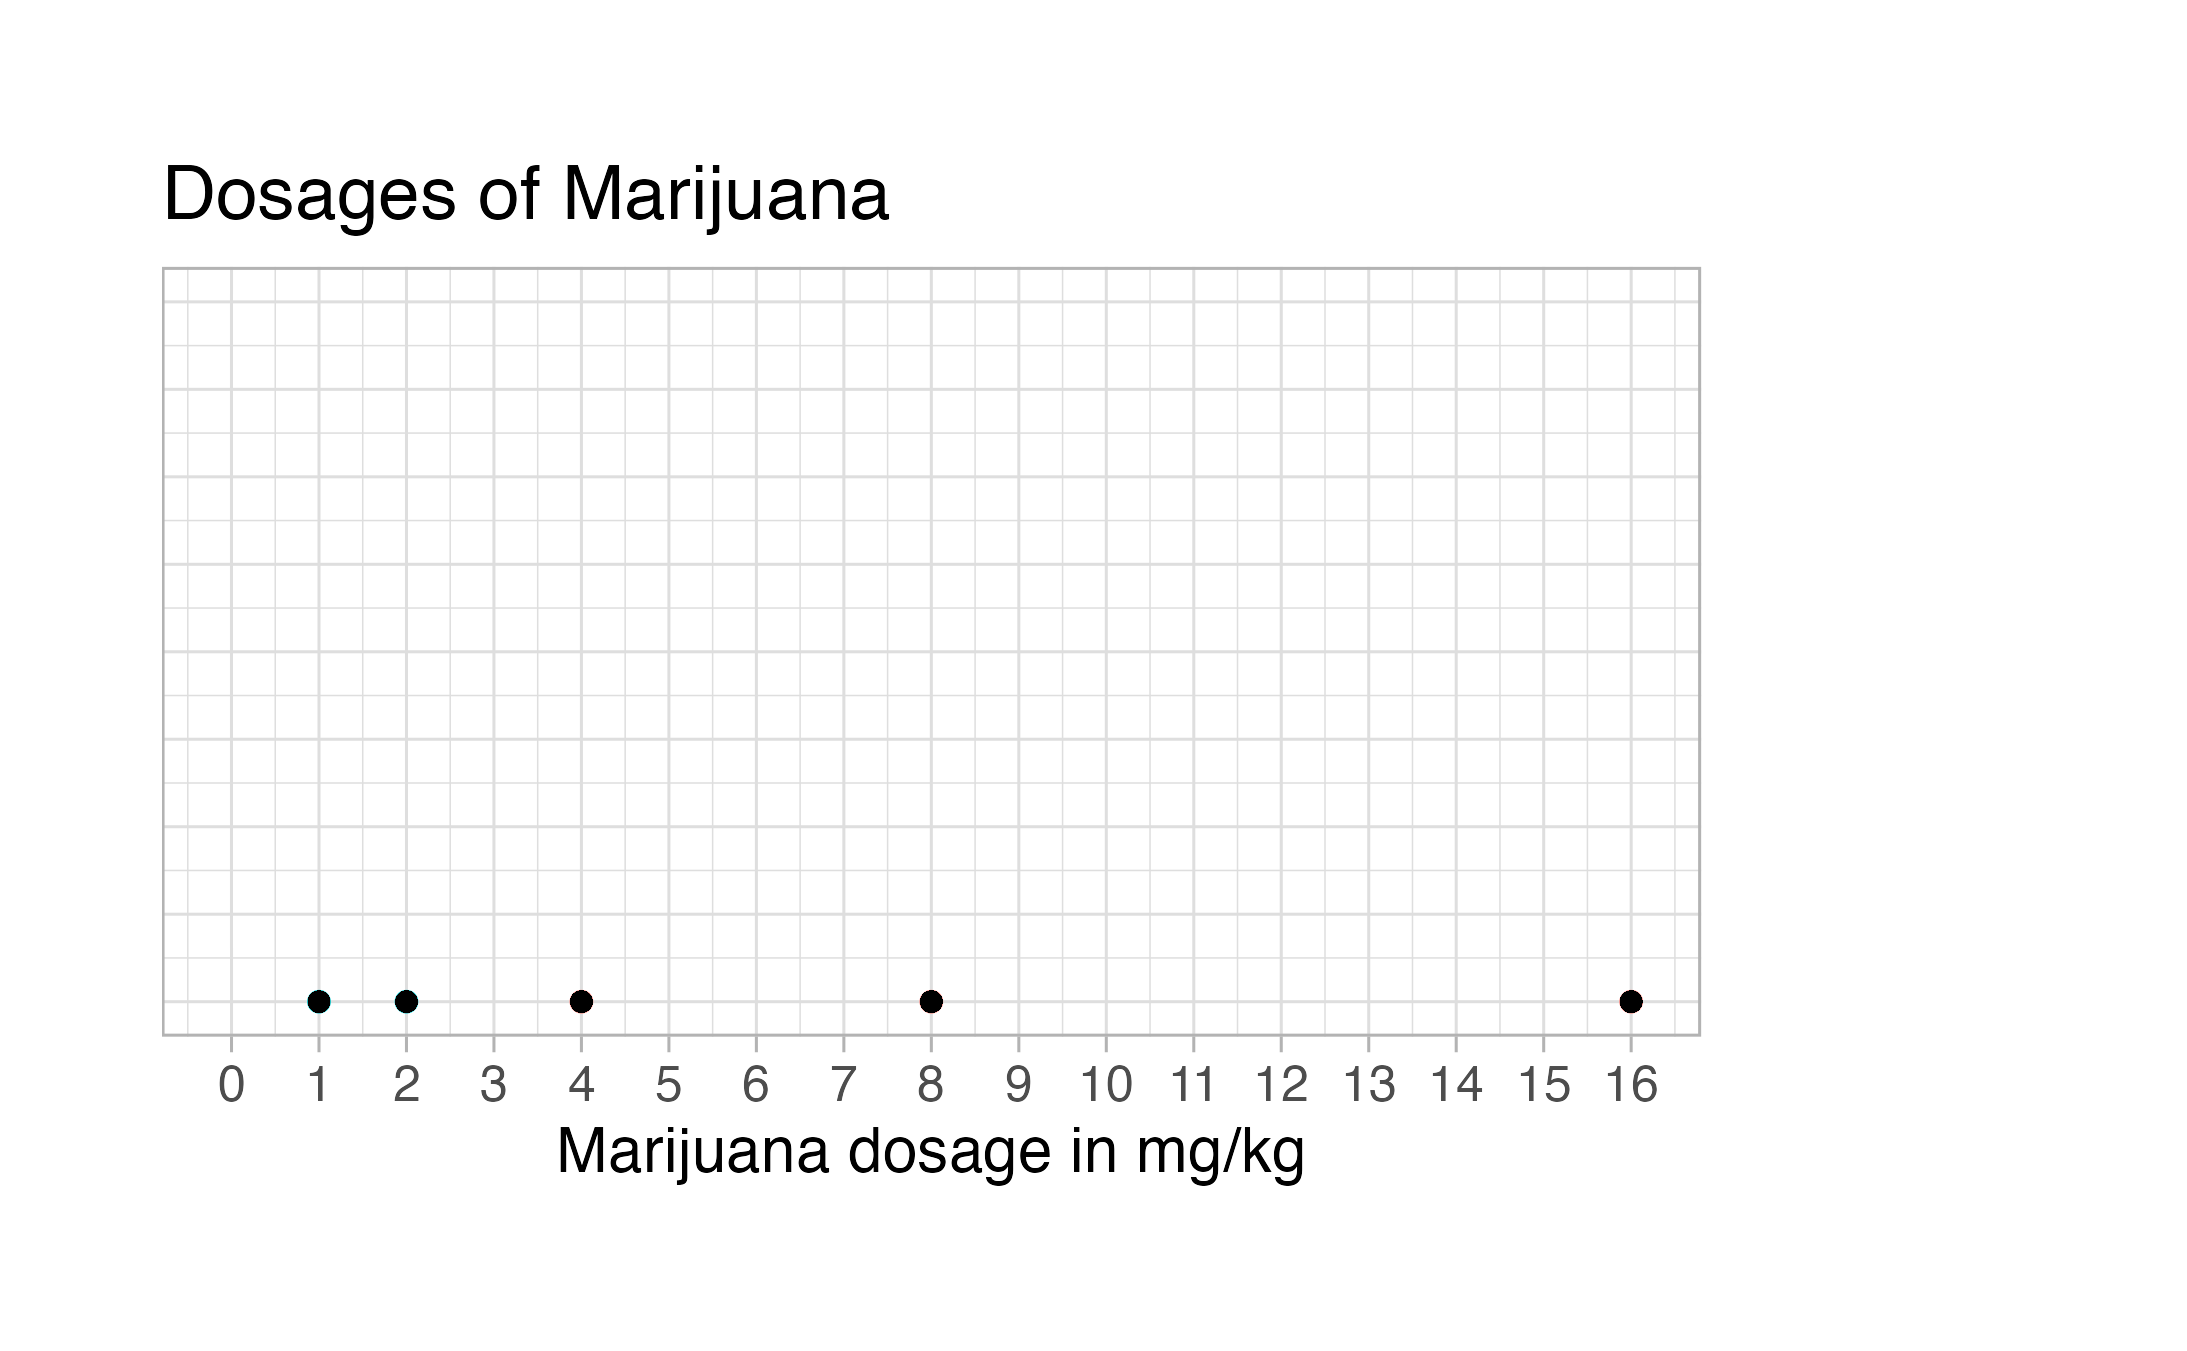
\includegraphics[scale=0.6]{iso1.png}
\end{center}
\end{frame}

\begin{frame}
\begin{center}
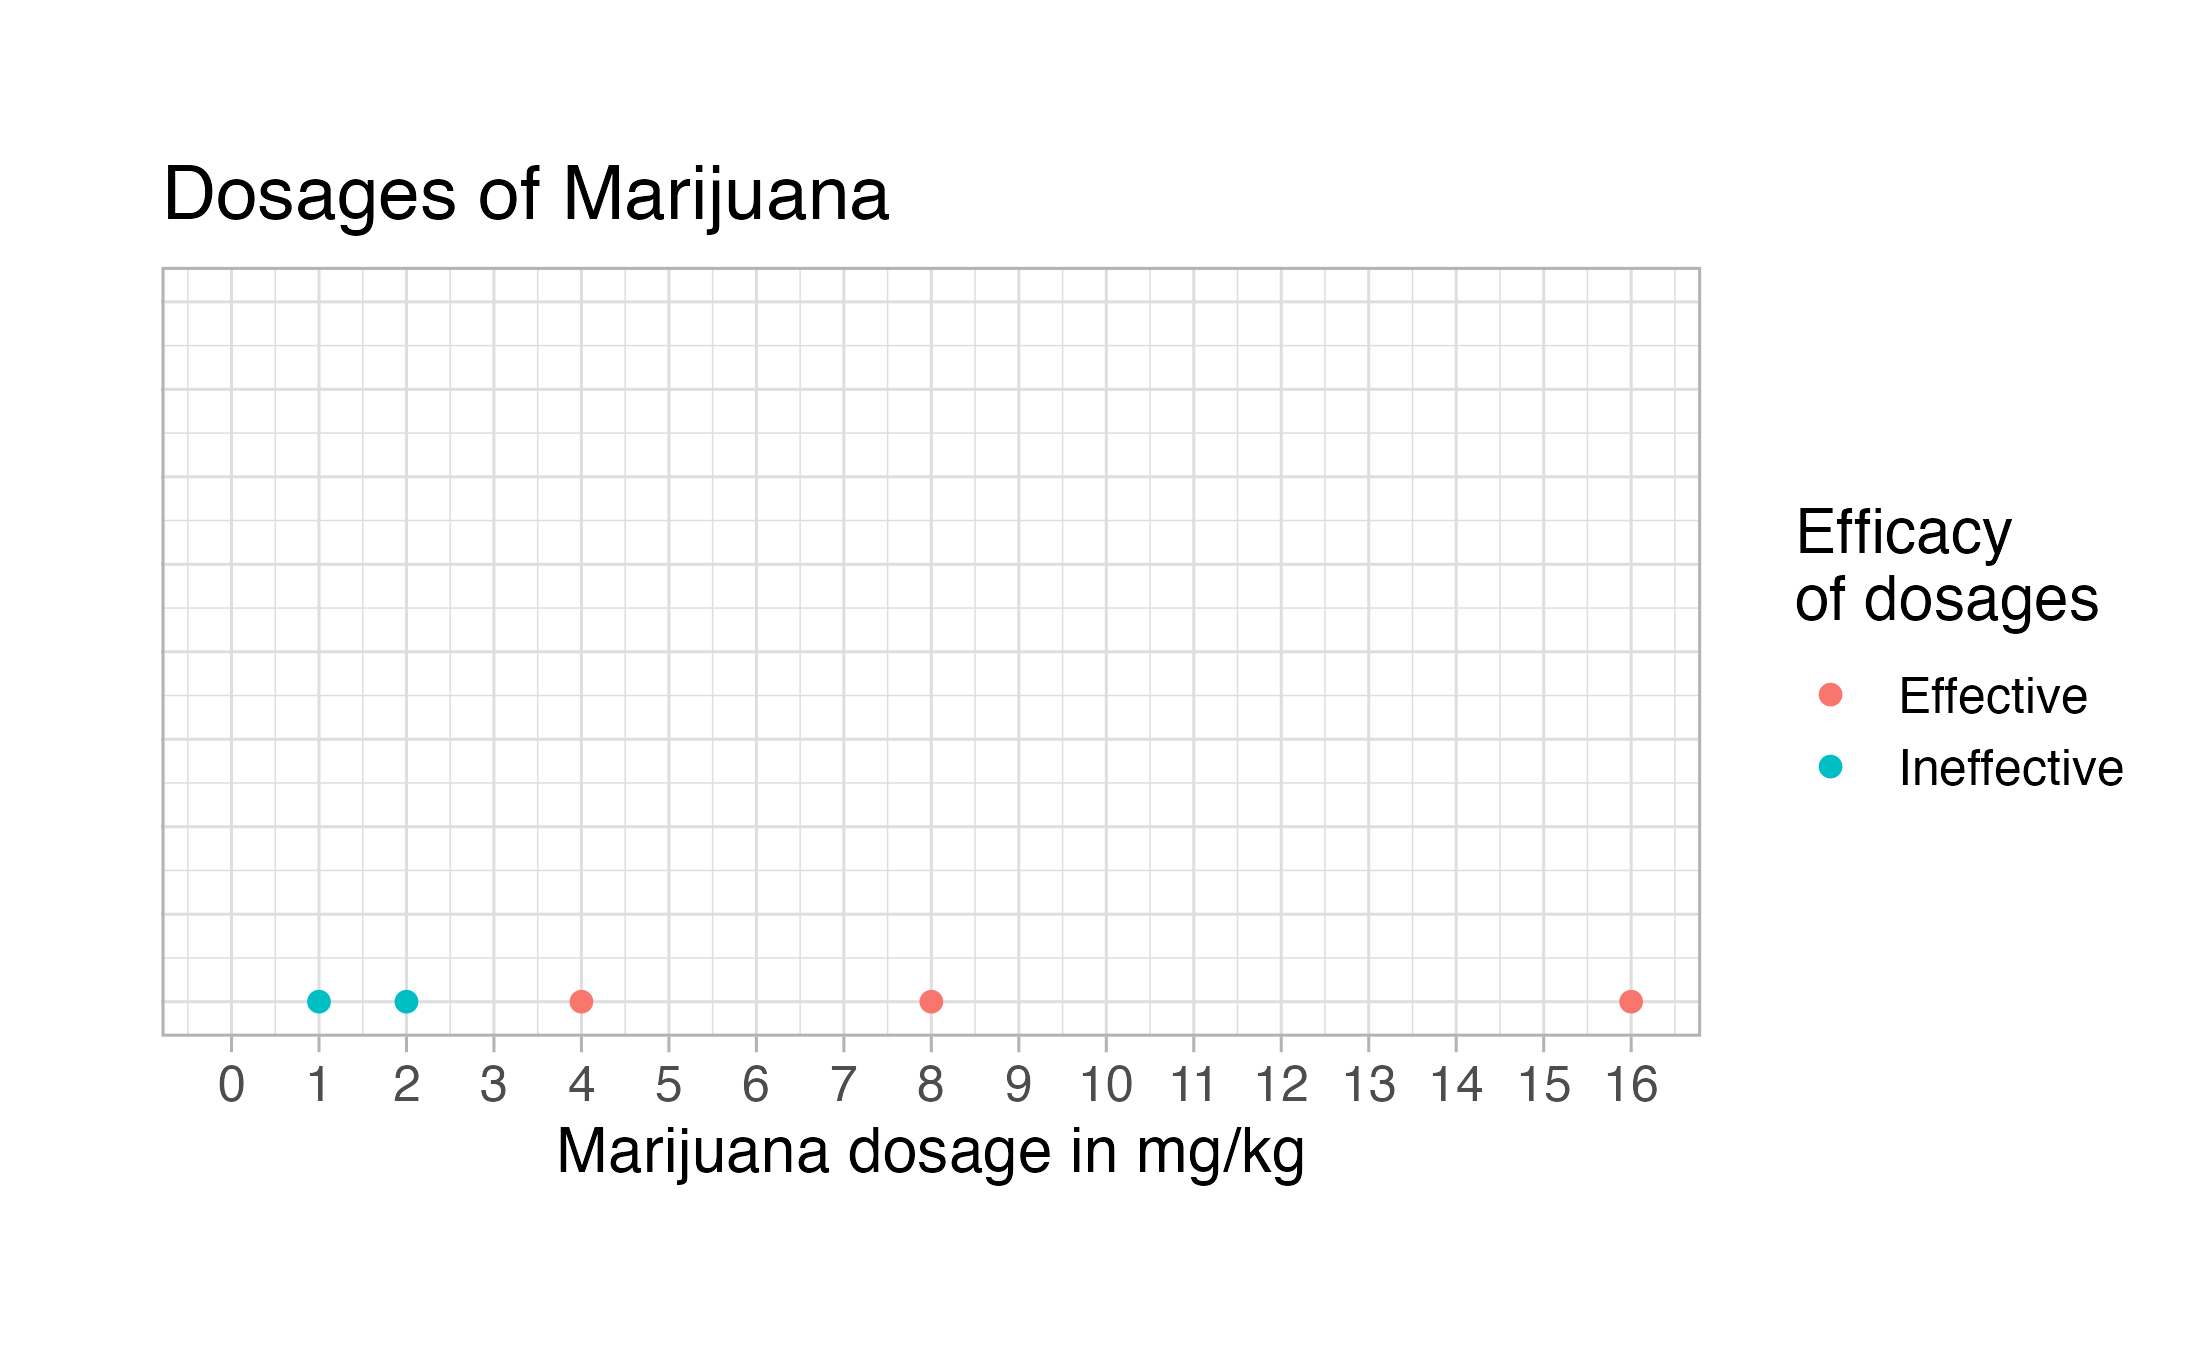
\includegraphics[scale=0.6]{iso2.png}
\end{center}
\end{frame}

\begin{frame}
\begin{center}
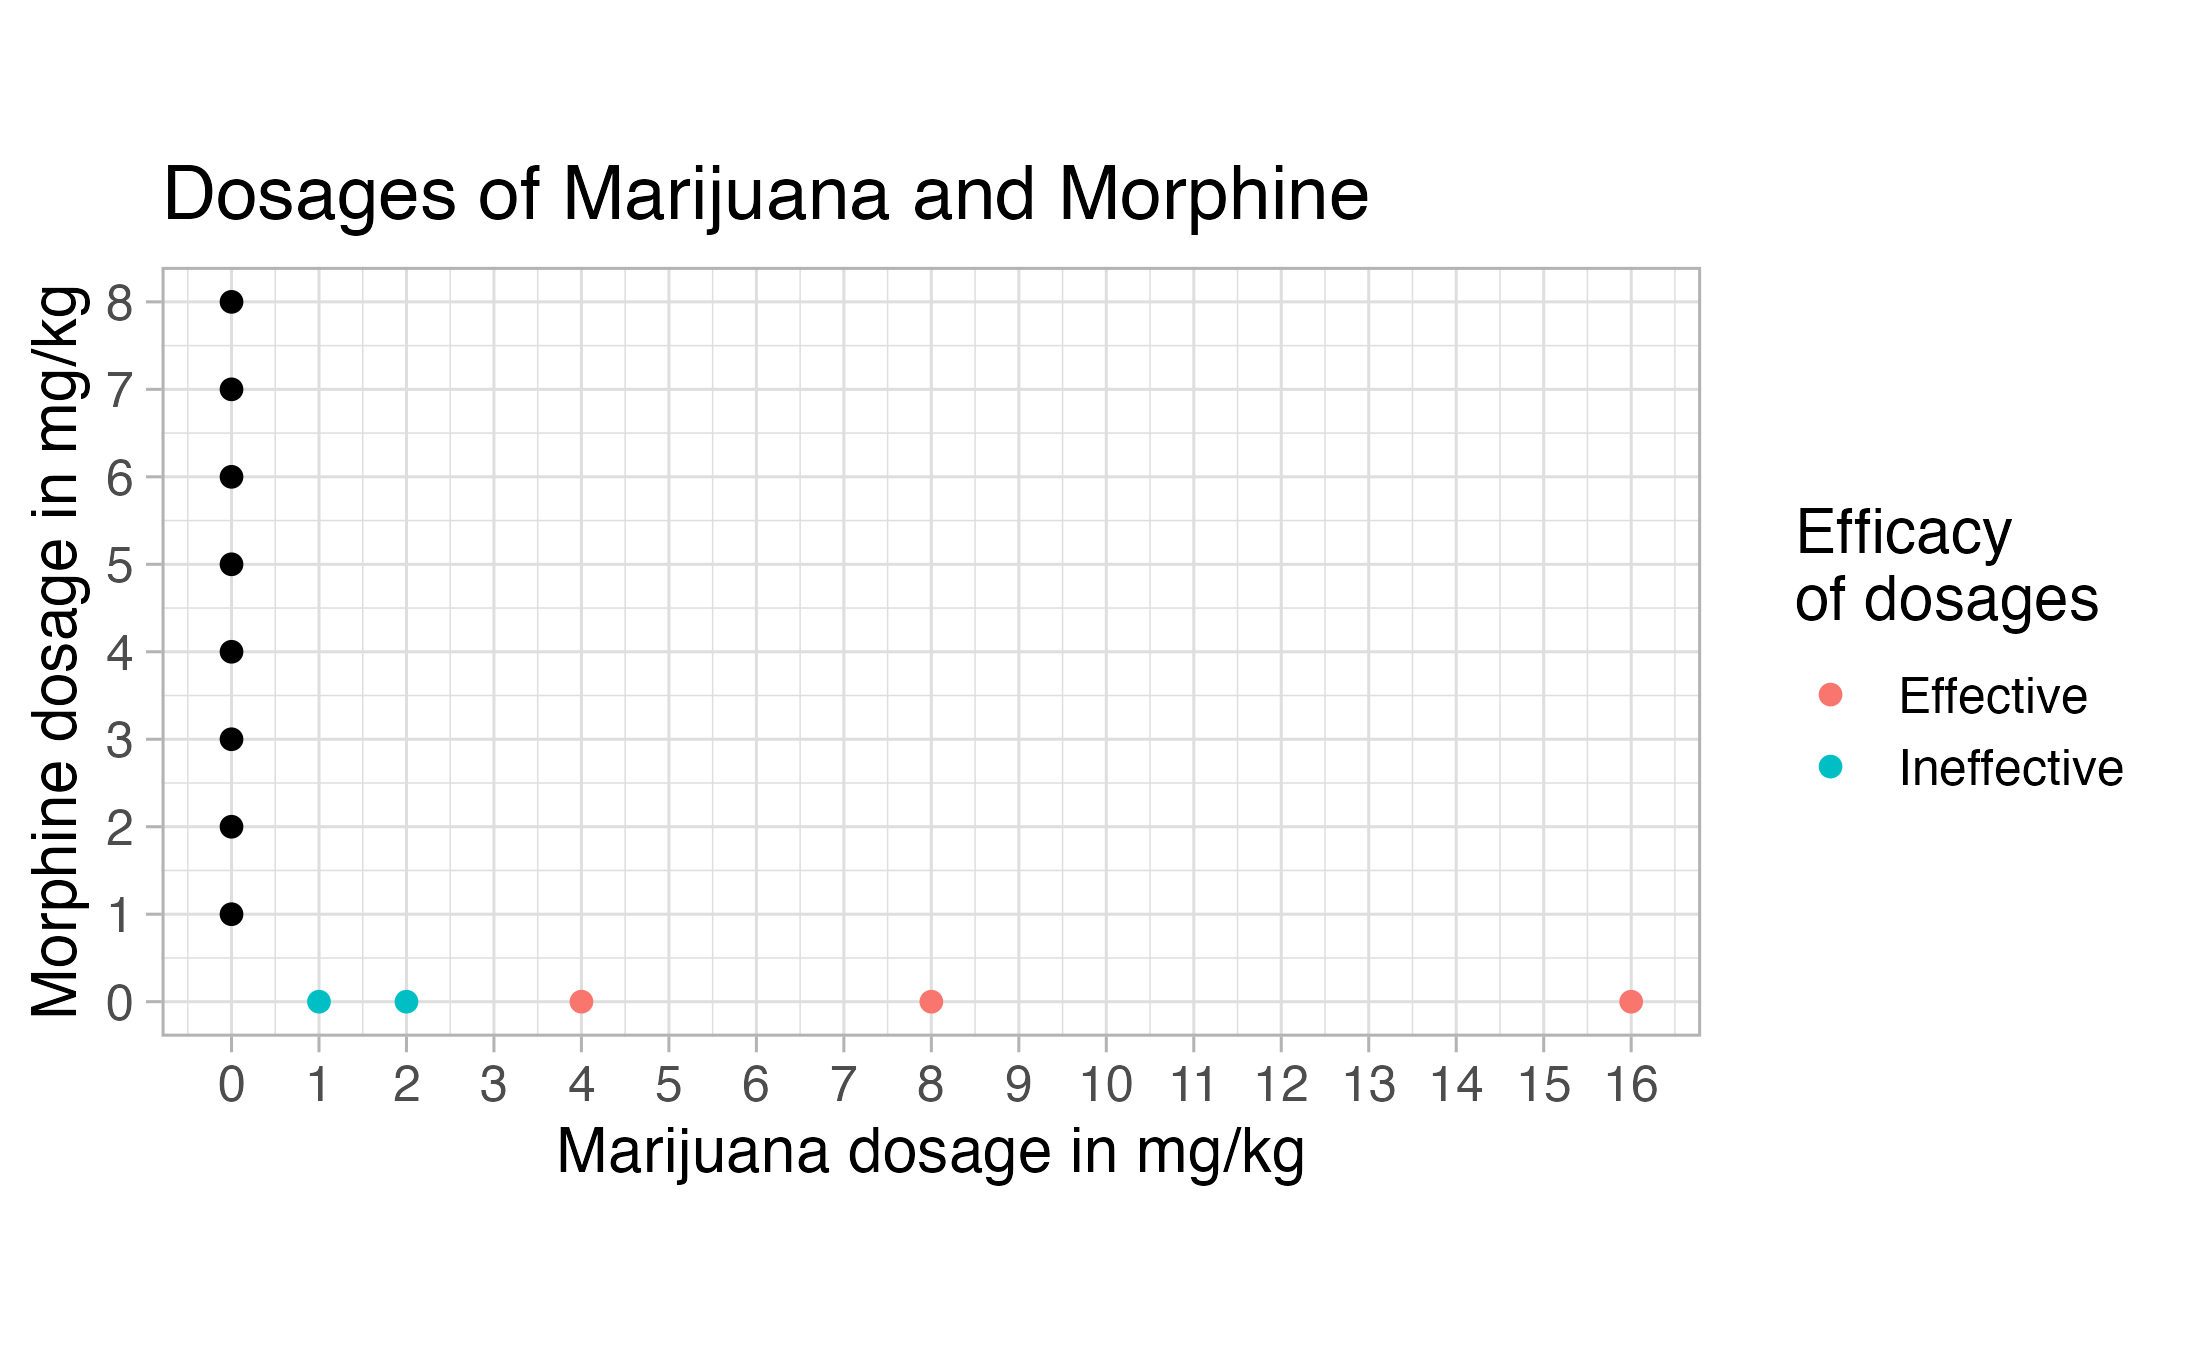
\includegraphics[scale=0.6]{iso3.png}
\end{center}
\end{frame}

\begin{frame}
\begin{center}
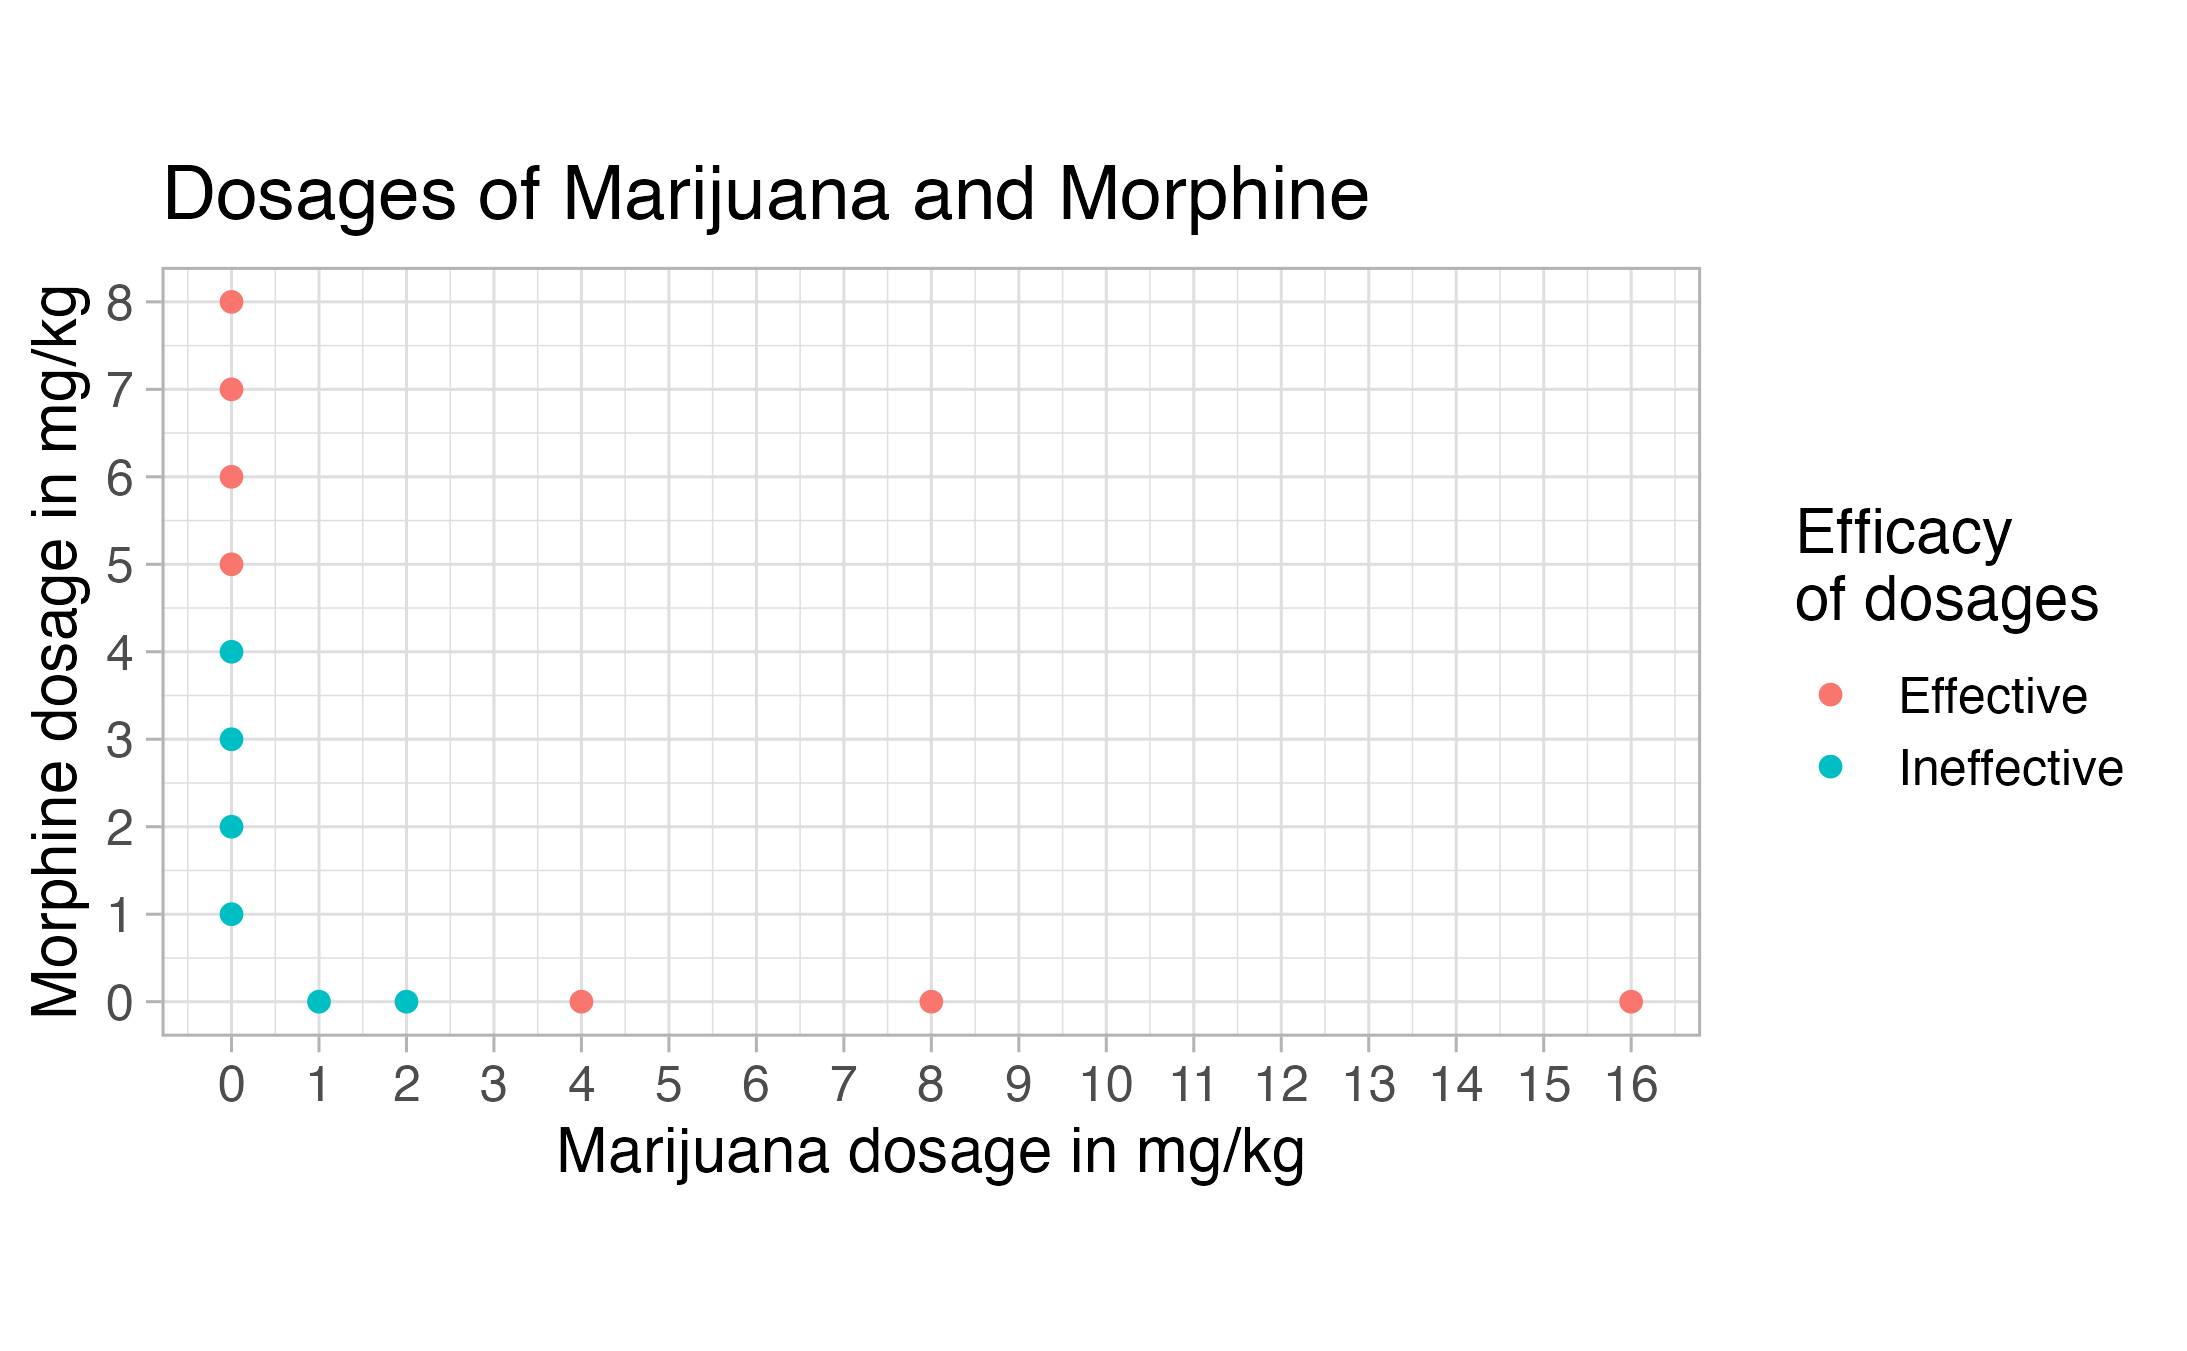
\includegraphics[scale=0.6]{iso4.png}
\end{center}
\end{frame}

\begin{frame}
\begin{center}
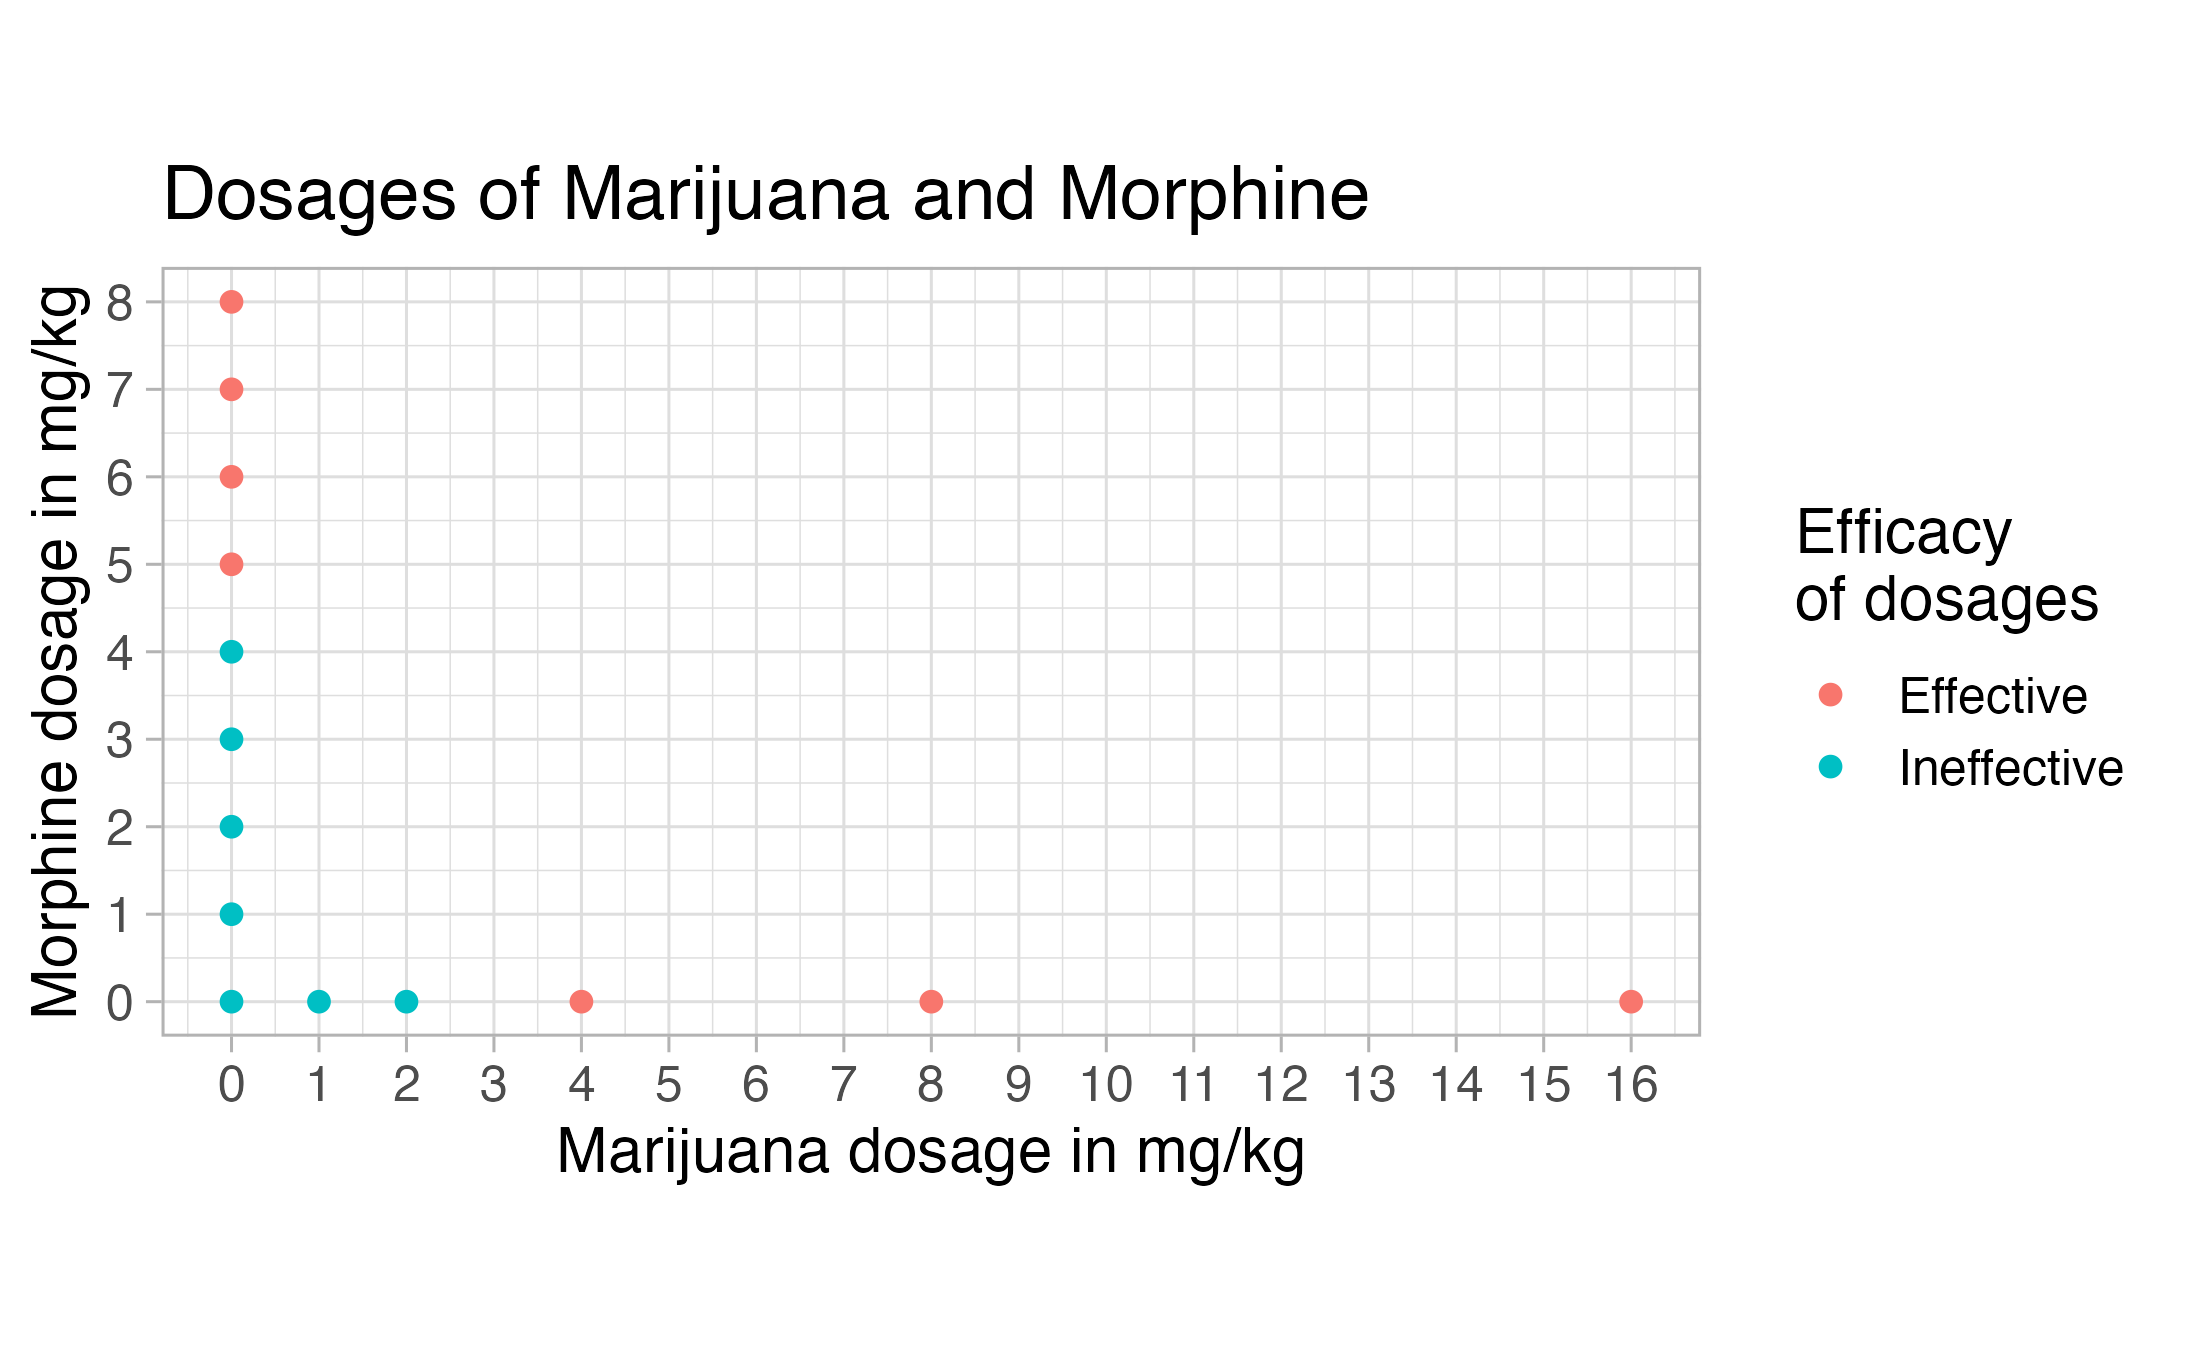
\includegraphics[scale=0.6]{iso5.png}
\end{center}
\end{frame}

\begin{frame}
\begin{center}
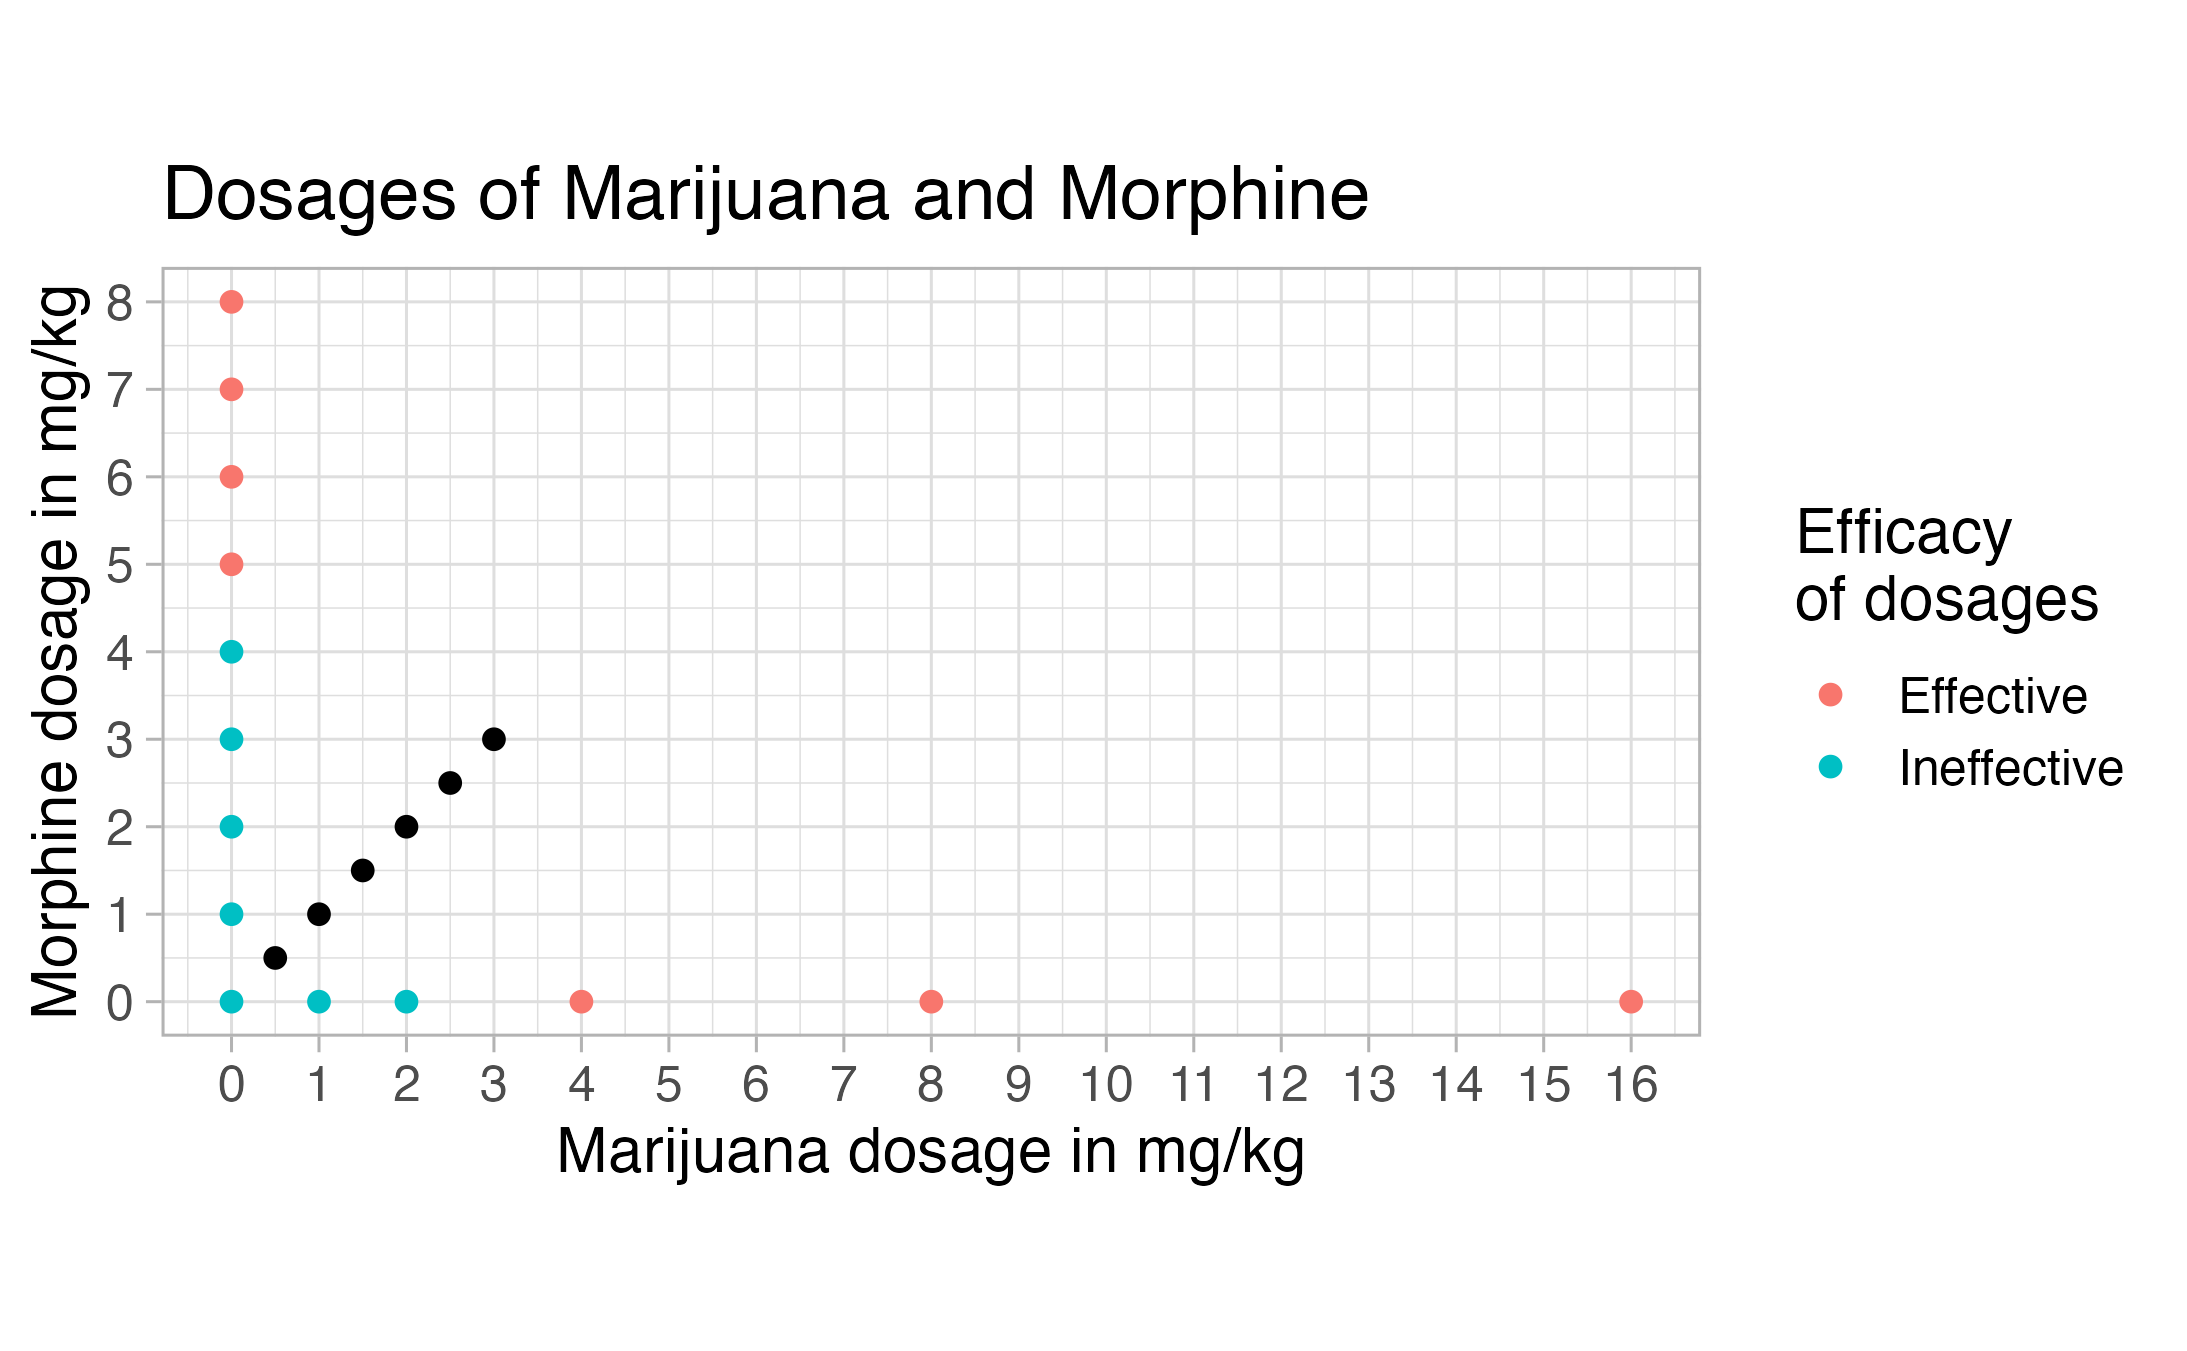
\includegraphics[scale=0.6]{iso6.png}
\end{center}
\end{frame}

\begin{frame}
\begin{center}
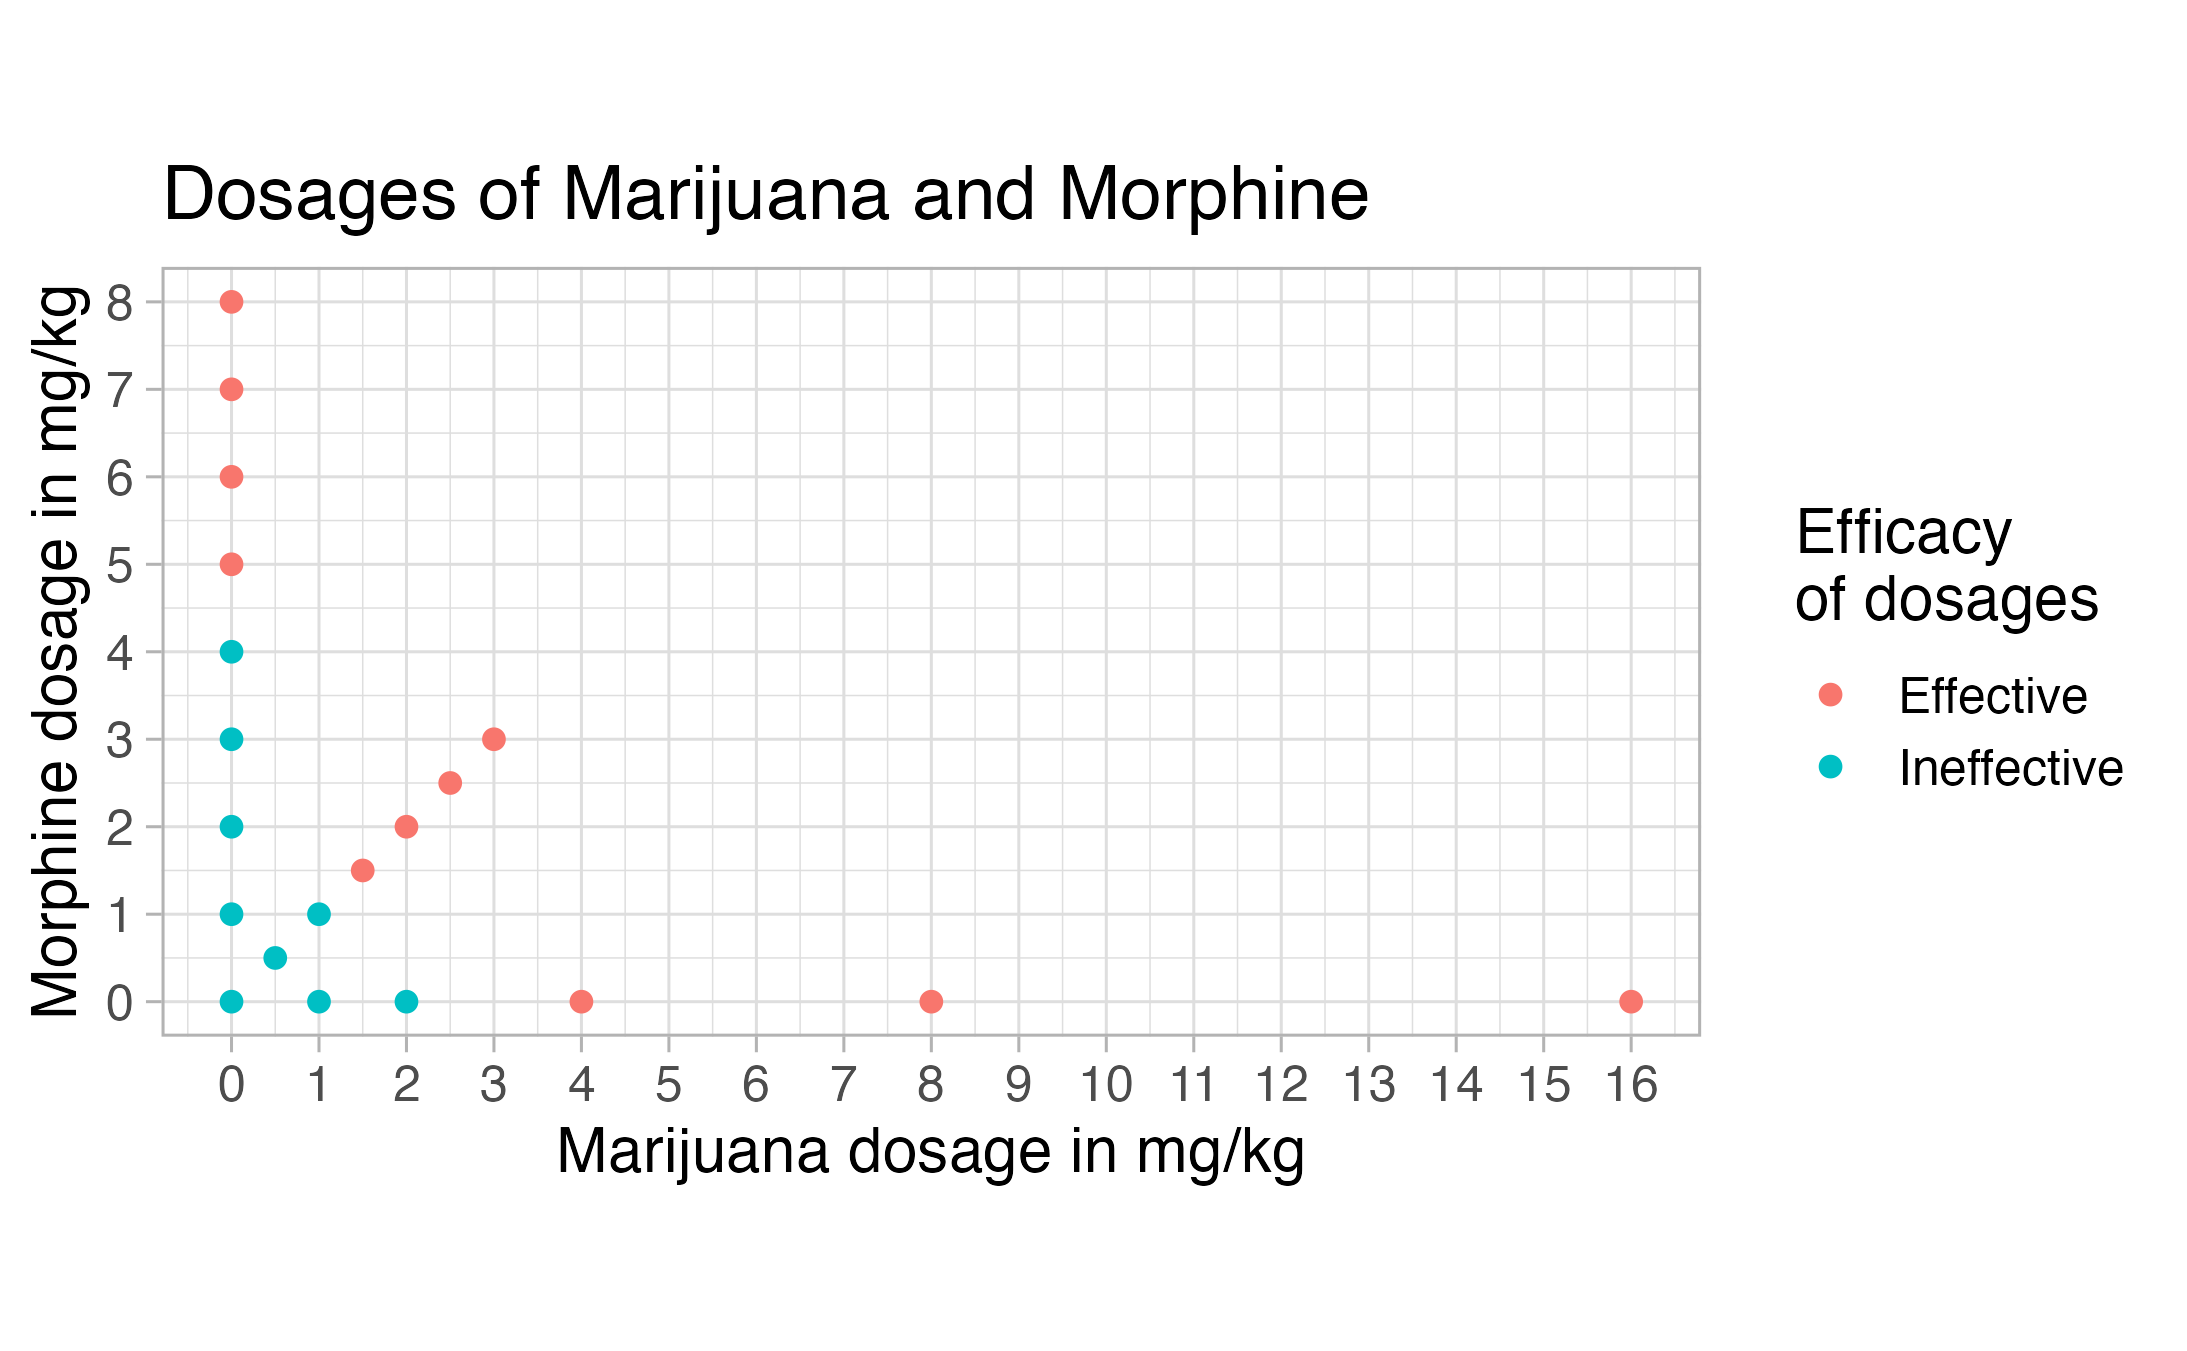
\includegraphics[scale=0.6]{dosages_plot.png}
\end{center}
\end{frame}

\begin{frame}
\begin{center}
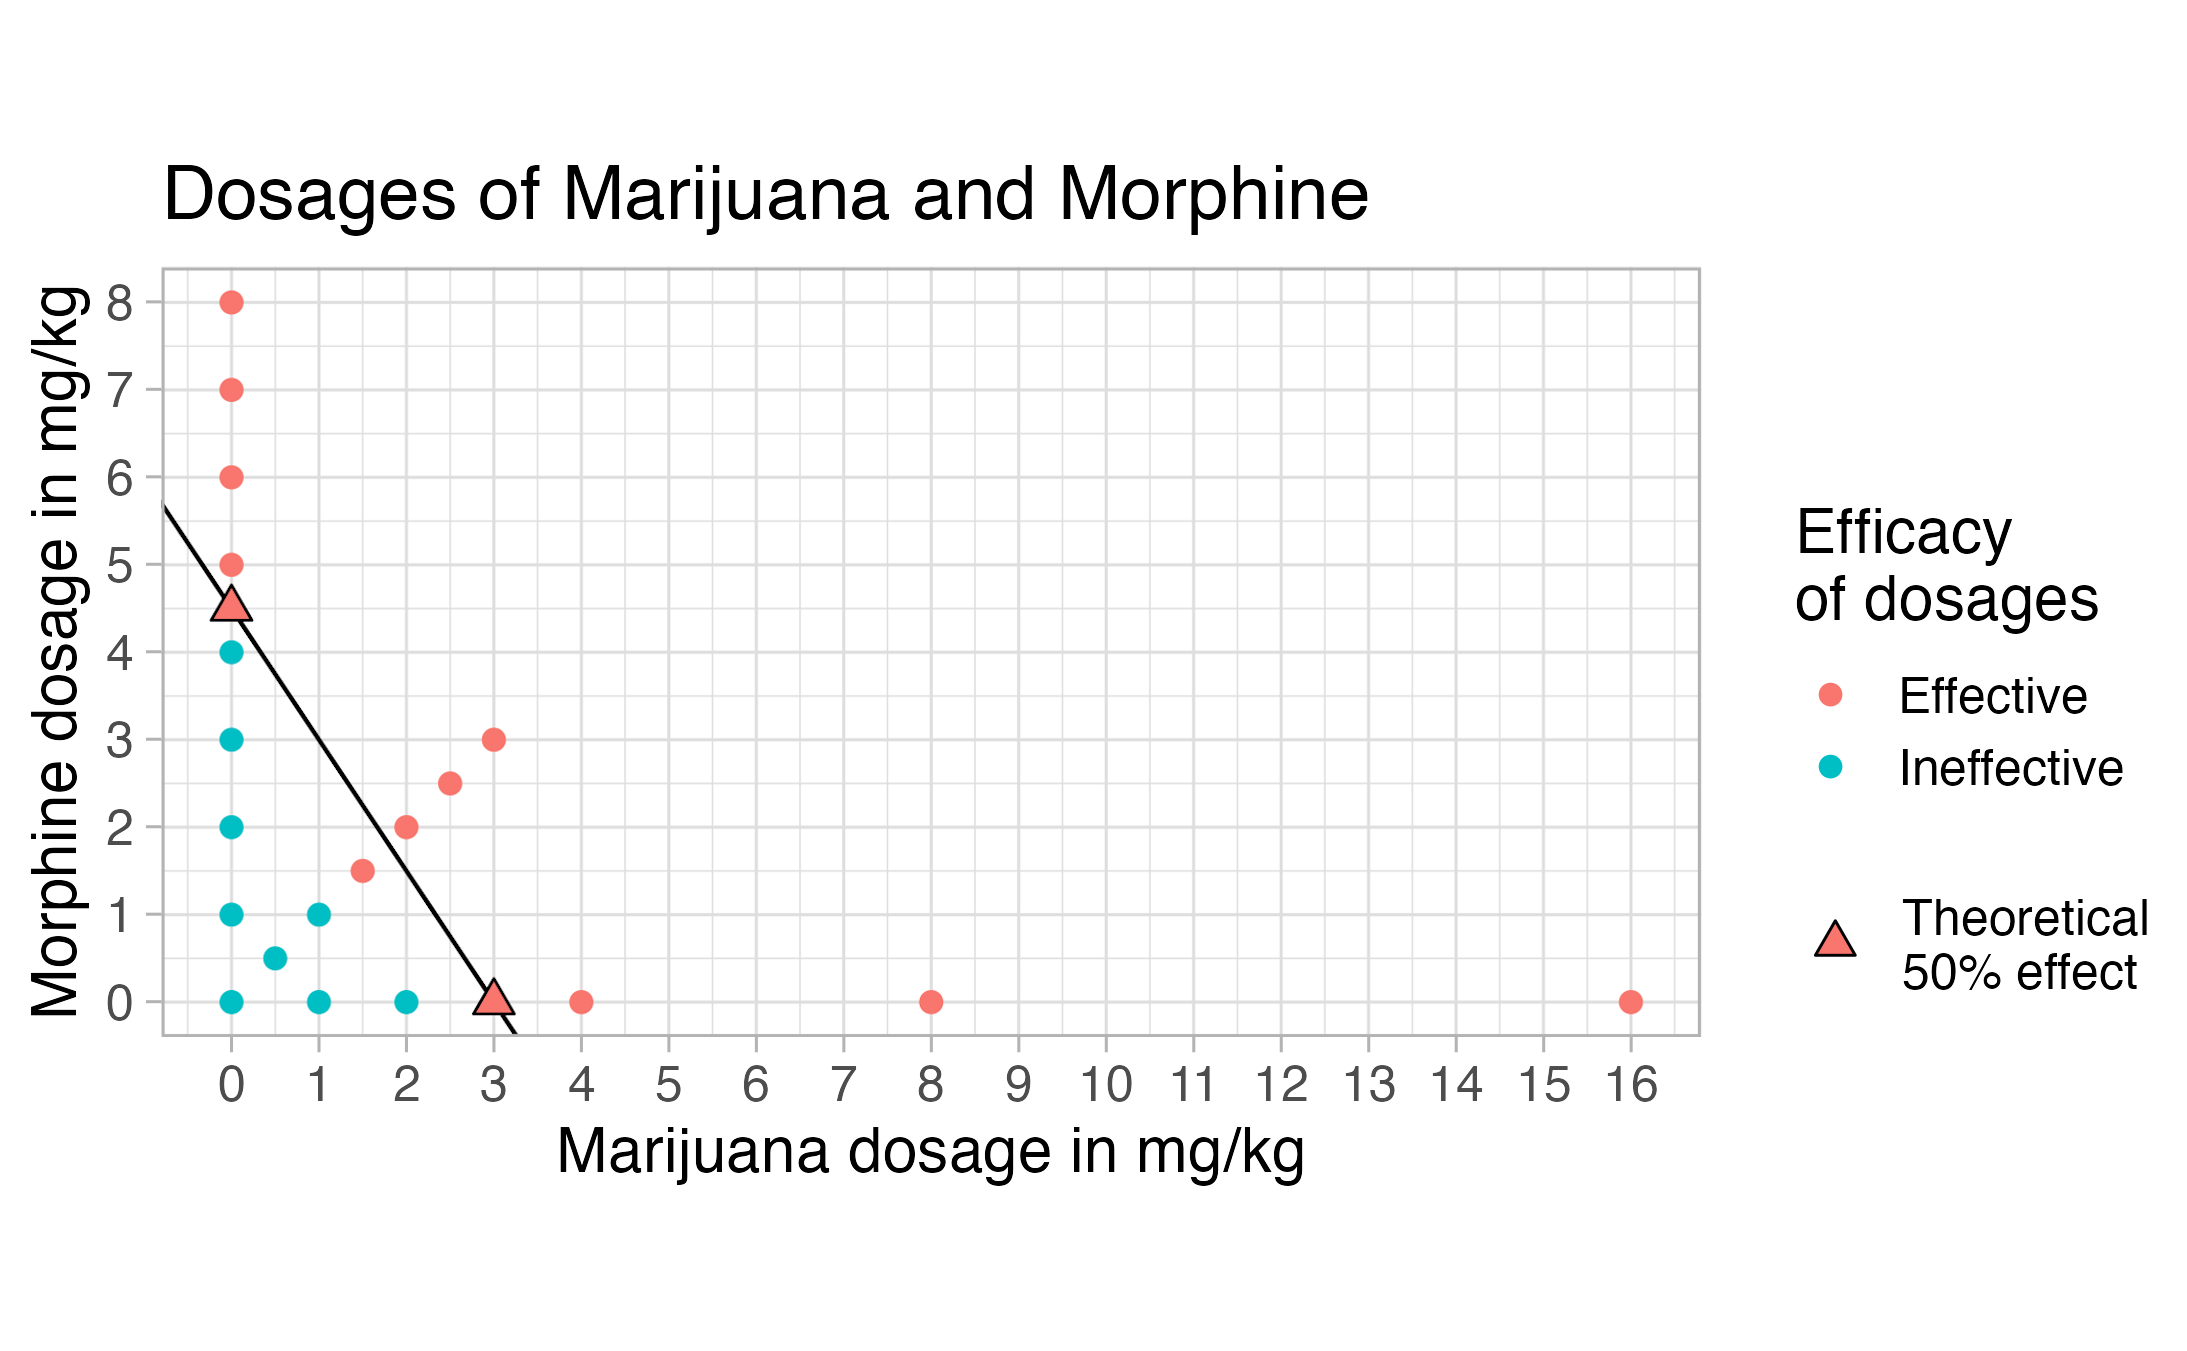
\includegraphics[scale=0.6]{isobole.png}
\end{center}
\end{frame}

\section{Isobole Insights}
\begin{frame}
\frametitle{Isobole Insights}
\begin{itemize}[label={$\blacktriangleright$}]
\item The isobole tests whether there is interaction between the two drugs.
\item If the drugs act independently, then all dosages on the isobole have an efficacy of 50\%.
\item All points above (resp. below) the isobole have an efficacy greater (resp. lesser) than 50\%.
\item A point below the isobole with an efficacy greater than 50\% is a departure from independence indicating synergy.
\end{itemize}
\end{frame}

\section{Isobole Conclusion}
\begin{frame}
\frametitle{Isobole Conclusion}
\begin{itemize}[label={\checkmark}]
\item \textbf{First objective, minimal effective dosage:} \\
\begin{itemize}[label={$\blacktriangleright$}]
\item 4.0 mg/kg for marijuana alone;
\item 5.0 mg/kg for morphine alone;
\item 1.5 mg/kg of each for both drugs.
\end{itemize}
\item \textbf{Second objective, synergy:} \\
Dosage of 1.5 mg/kg for both drugs has a \textbf{potential} to be synergistic.
\end{itemize}
\end{frame}

\section{Isobole Method Assumptions}
\begin{frame}
\frametitle{Isobole Method Assumptions}
\textbf{Constant potency level}

For any chosen efficacy level, the ratio between the dosages of morphine and marijuana must remain the same.
\end{frame}

\begin{frame}
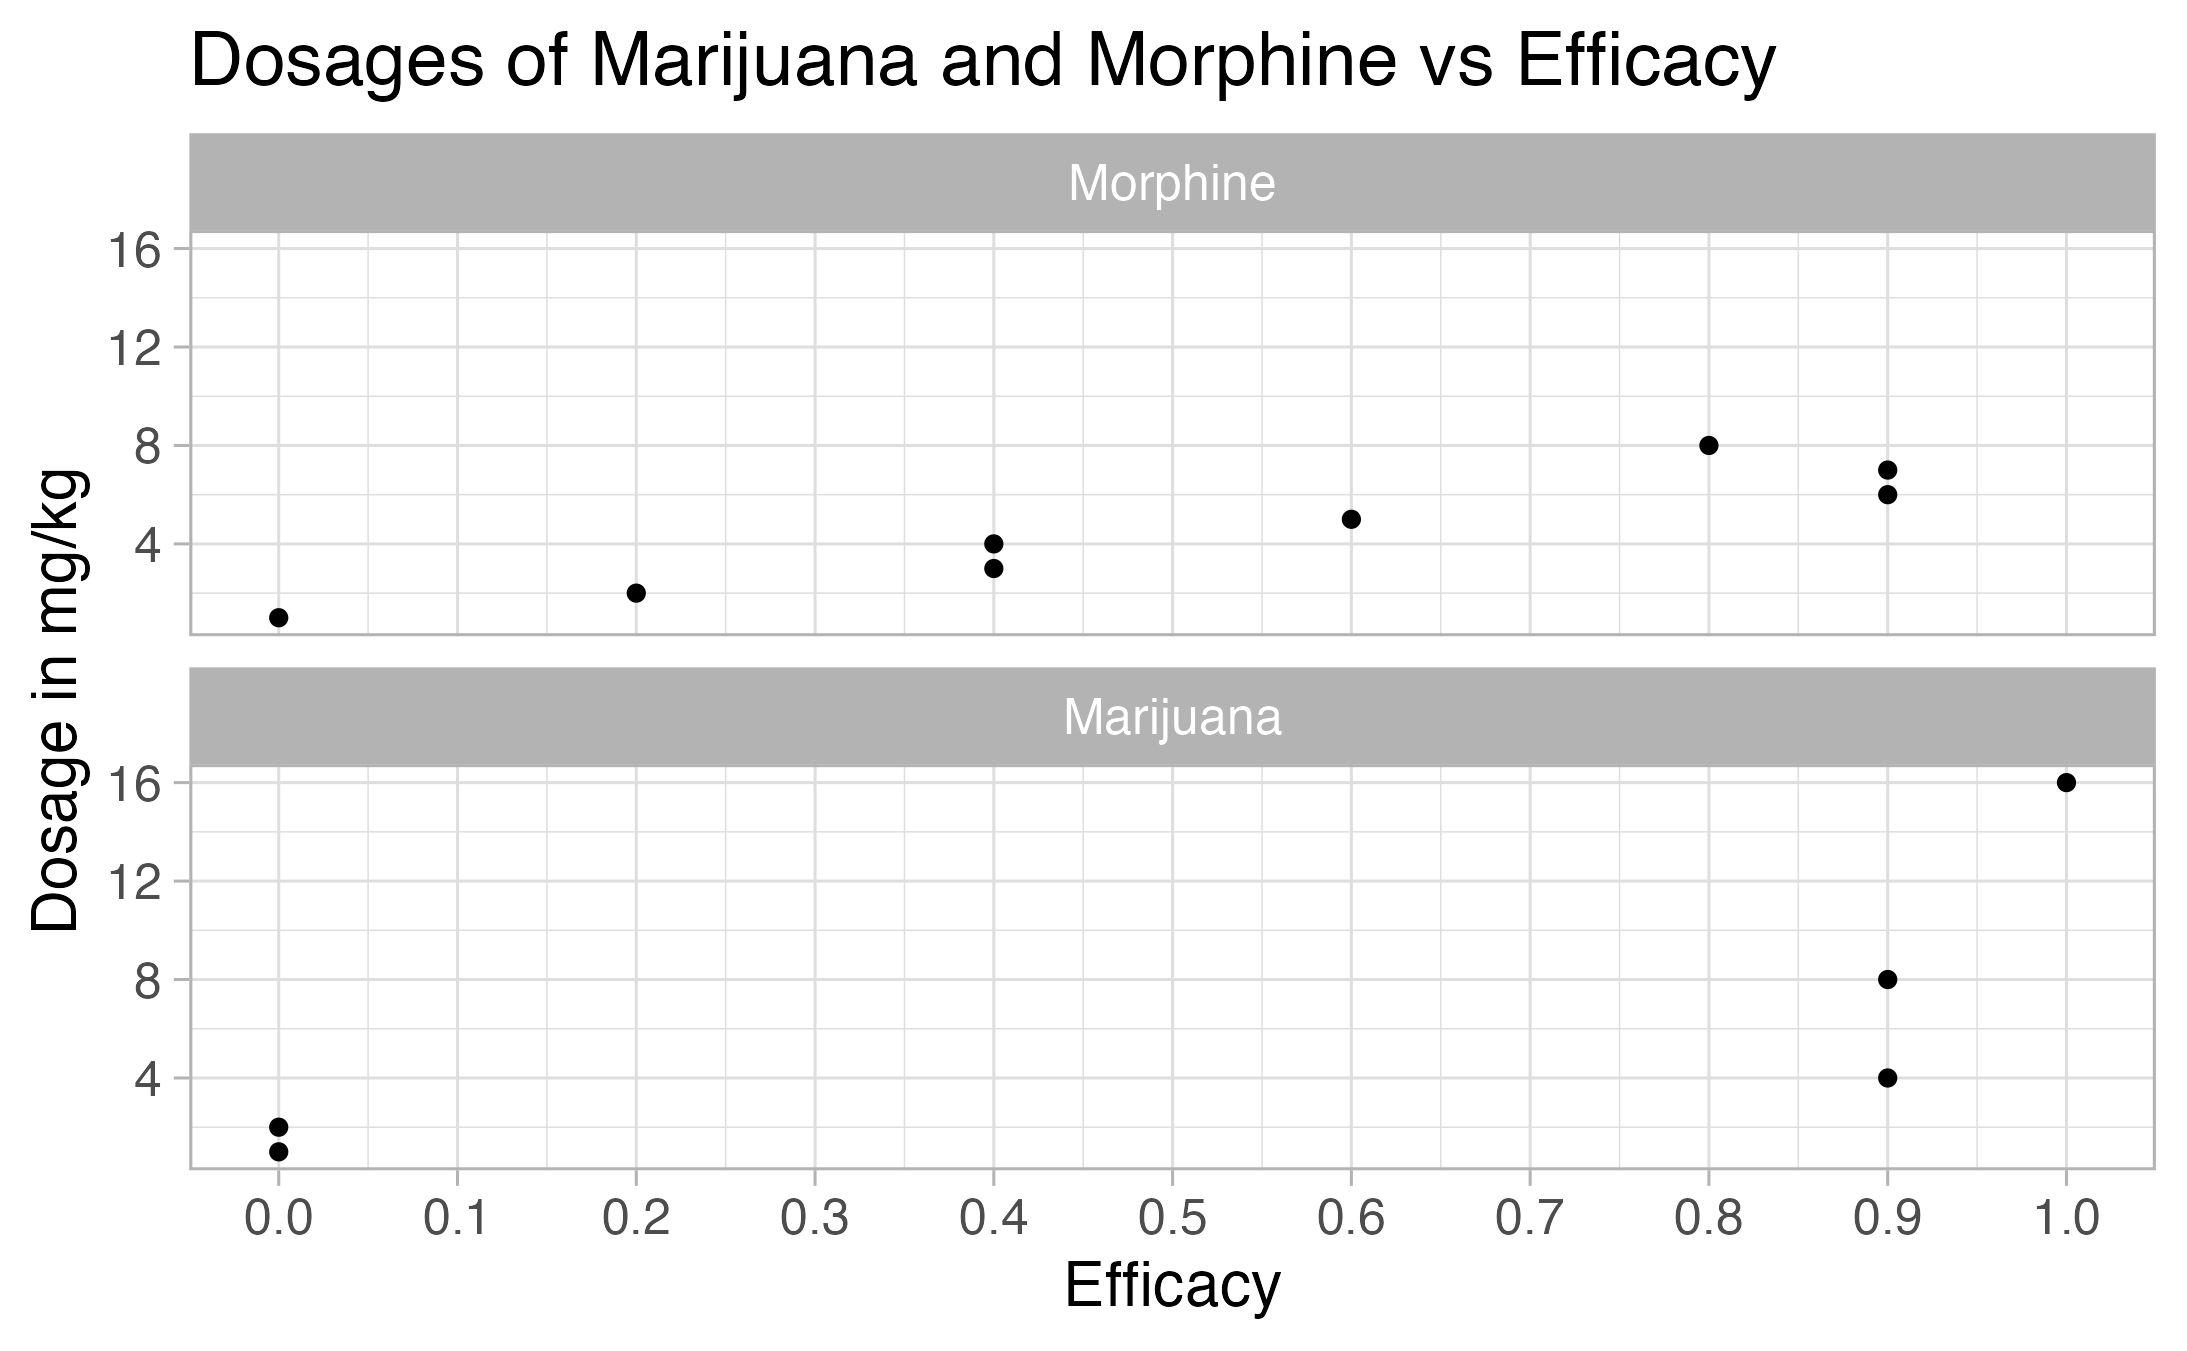
\includegraphics[scale=0.6]{potency_ratio.png}
\end{frame}

\begin{frame}
\begin{itemize}[label={$\blacktriangleright$}]
\item Only two common efficacy levels, 0.0 and 0.9
\item This is not enough to verify the assumption for this experiment.
\item This weakness is due to dosage choices for marijuana.
\item However, the linear isobole method is used in multiple experiments which are extremely similar.
\end{itemize}
\end{frame}

\begin{frame}
\textbf{Choice of theoretical dosages with 50\% efficacy}

For morphine:
\begin{itemize}[label={$\blacktriangleright$}]
\item chosen between 4 and 5 mg/kg;
\item this represents an interval of 1 mg/kg;
\item effect level is between 40\% and 60\%.
\end{itemize}
For marijuana:
\begin{itemize}[label={$\blacktriangleright$}]
\item chosen between 2 and 4 mg/kg;
\item this represents an interval of 2 mg/kg;
\item effect level is between 0\% and 90\%.
\end{itemize}
\end{frame}

\begin{frame}
\begin{itemize}[label={$\blacktriangleright$}]
\item The 50\% efficacy dosage for marijuana cannot be pinpointed because of the chosen dosages of marijuana in the experiment.
\item Finding that dosage would mean finding a better minimal effective dosage, which could result in costs reduction.
\item The position of that dosage could move the isobole significantly, making it more or less strict towards synergistic dosages.
\end{itemize}
\end{frame}

\begin{frame}
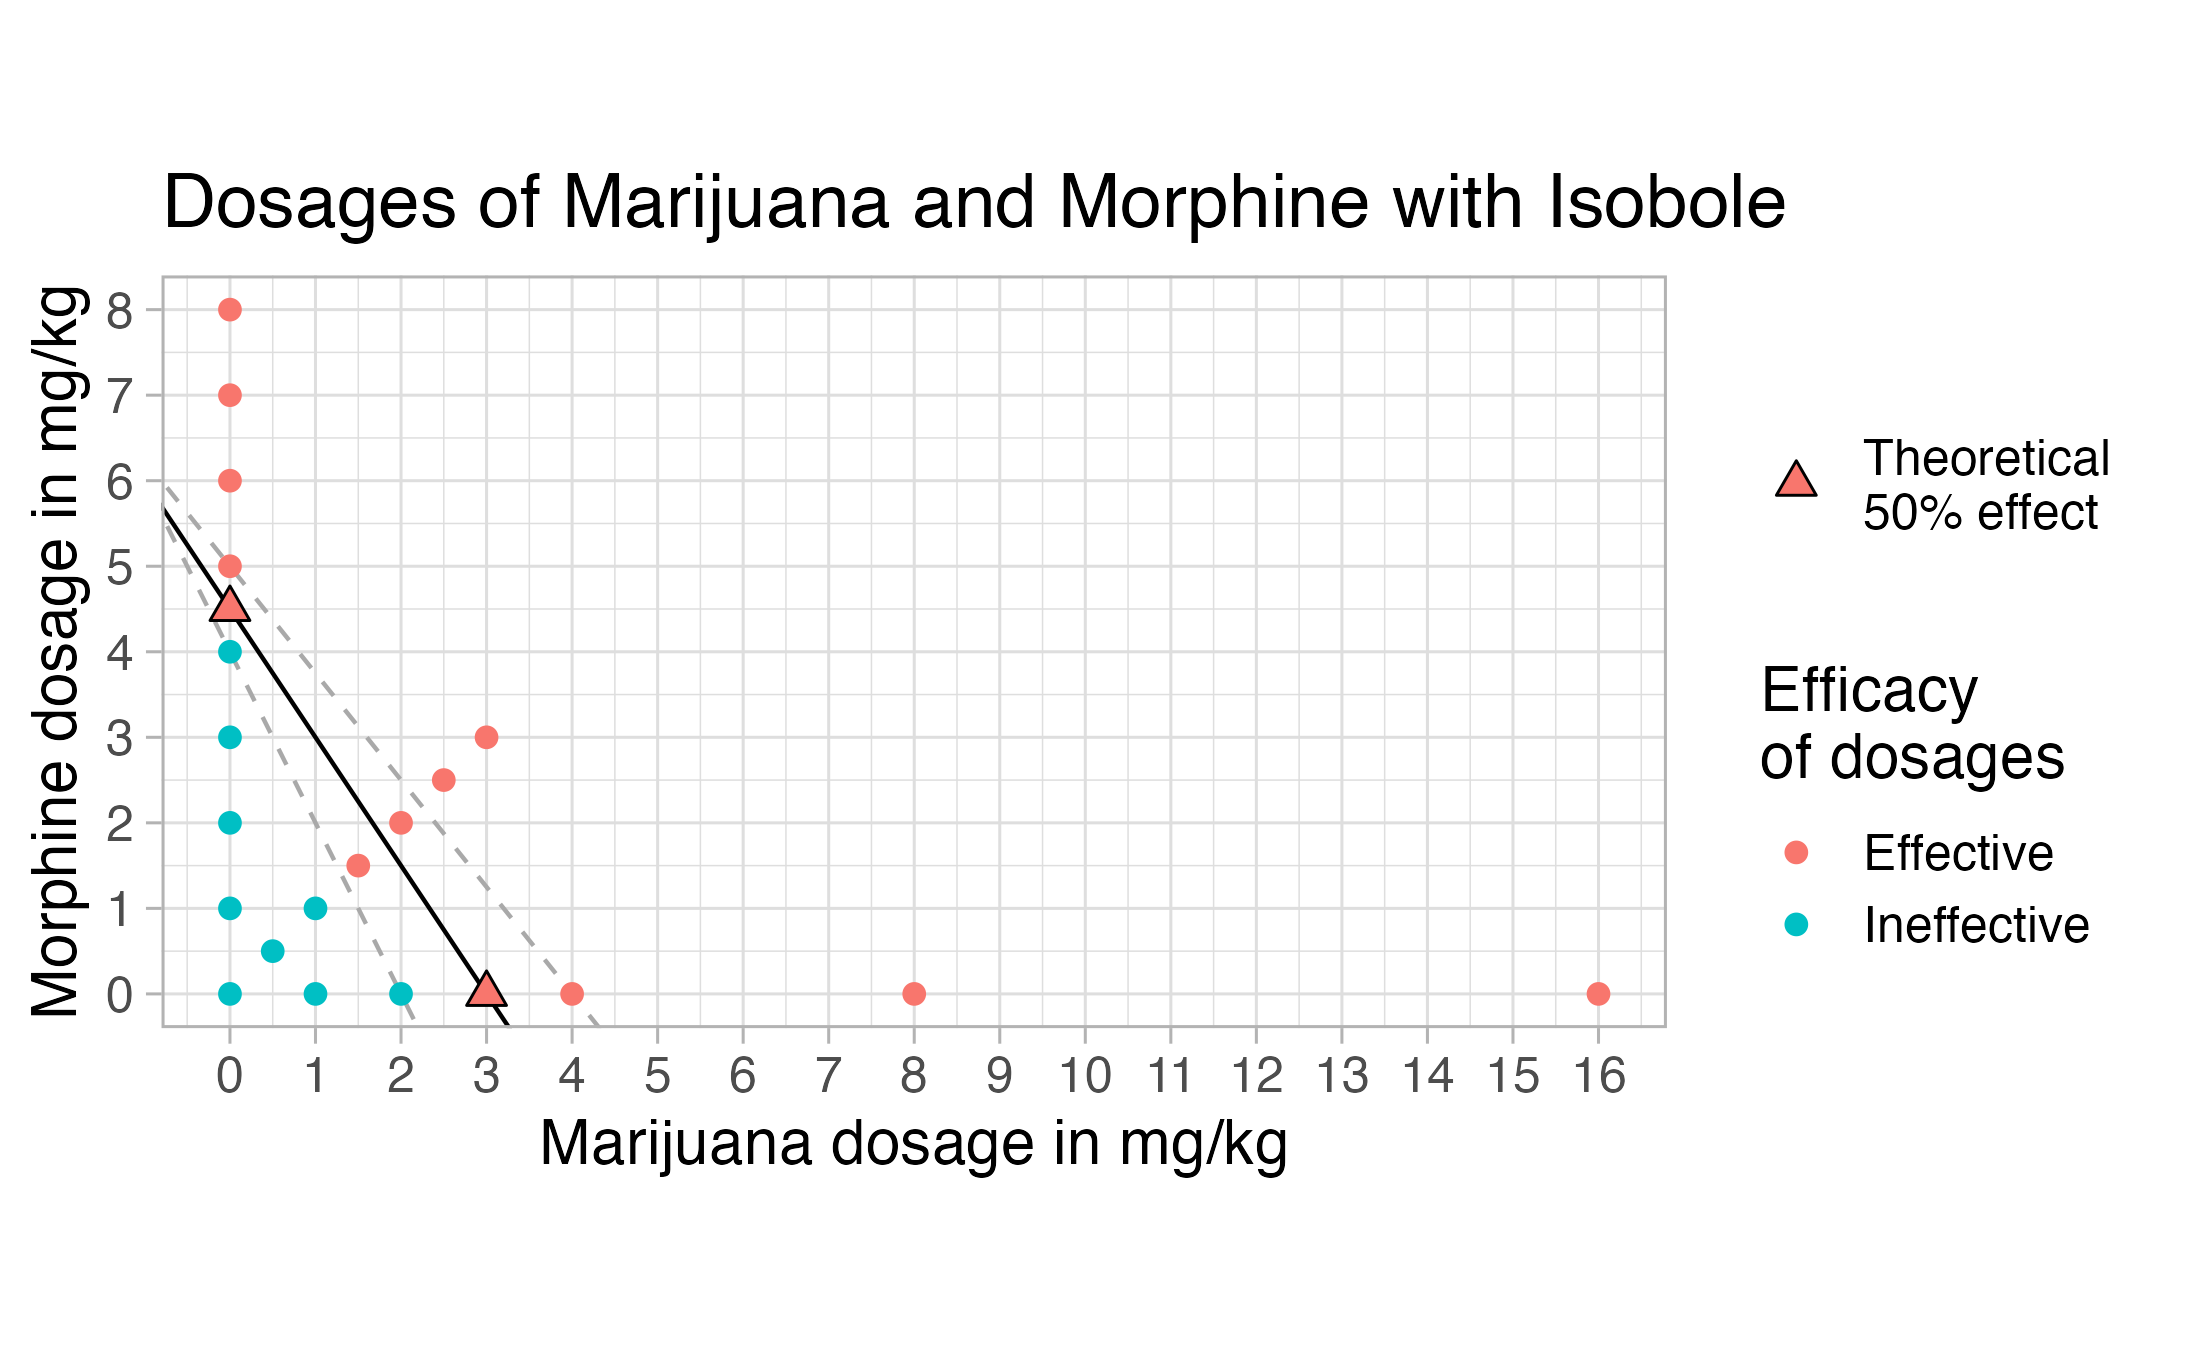
\includegraphics[scale=0.6]{isobole-vary.png}
\end{frame}

\section{Recommendations}

\begin{frame}
\frametitle{Recommendations}
\begin{itemize}[label={\checkmark}]
\item \textbf{Complete the experiment with trials for at least 4 dosages of marijuana between 2.0 and 4.0 mg/kg.}
\item Experiment with more dosages of morphine between 4.0 and 5.0 mg/kg.
\item Experiment with unequal amounts of marijuana and morphine to find other potential synergies.
\end{itemize}
\end{frame}

\section{Conclusion}
\begin{frame}
\frametitle{Conclusion}
\begin{itemize}[label={$\blacktriangleright$}]
\item Minimal effective dosages have been identified, but there could be significative improvement for marijuana.
\item One dosage combination has the potential to be synergistic, but only further experimentation will determine if it is the case.
\end{itemize}
\end{frame}

\begin{frame}
\frametitle{Q\&A Session}
Thank you for your attention. 

\bigskip

Feel free to ask us any question!
\end{frame}

\end{document}